\subsection{Gateway}
	Un \textit{gateway} è una componente localizzata all'interno di un'azienda che permette di rendere uniforme l'interfaccia di accesso ai dati dei singoli dispositivi configurati all'interno del gateway stesso.
	\newline
	Dai gateway è possibile inoltre configurare funzioni di accumulo dei pacchetti contenenti i dati dei sensori o di impostare alcuni timer, al termine dei quali deve essere effettuato l'invio dei dati all'interno dei rispettivi topic di Kafka.
	\newline
	Tutte le configurazioni vengono ricevute tramite appositi topic adibiti esclusivamente a questa funzione.
	\begin{itemize}
		\item La componente è stata sviluppata in Java 11.
	\end{itemize}
	
	\subsubsection{Diagramma dei package}%%%%%%%%%%%%OK
	  	\begin{figure}[H]
			\centering
			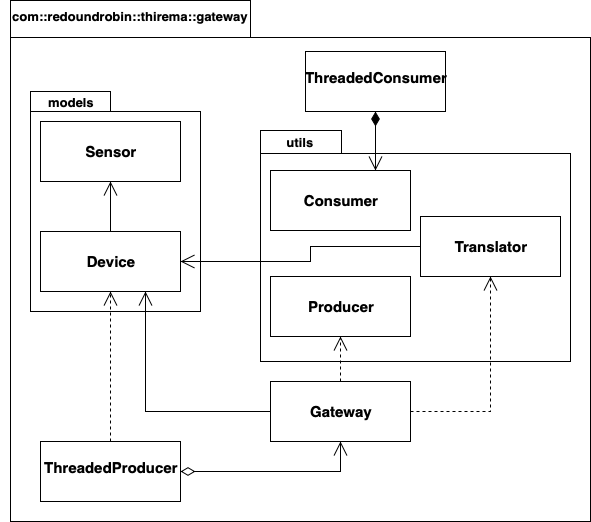
\includegraphics[scale=0.550]{res/images/GATEWAY/GatewayPackage.png}
			\caption{Diagramma dei package per la componente gateway}
			\label{Diagramma 1}
		\end{figure}
		\newpage		

	\begin{landscape}
		\subsubsection{Diagramma delle classi}%%%%%%%%%%%%%%%%%%%%%%%OK
		  	\begin{figure}[H]
				\centering
				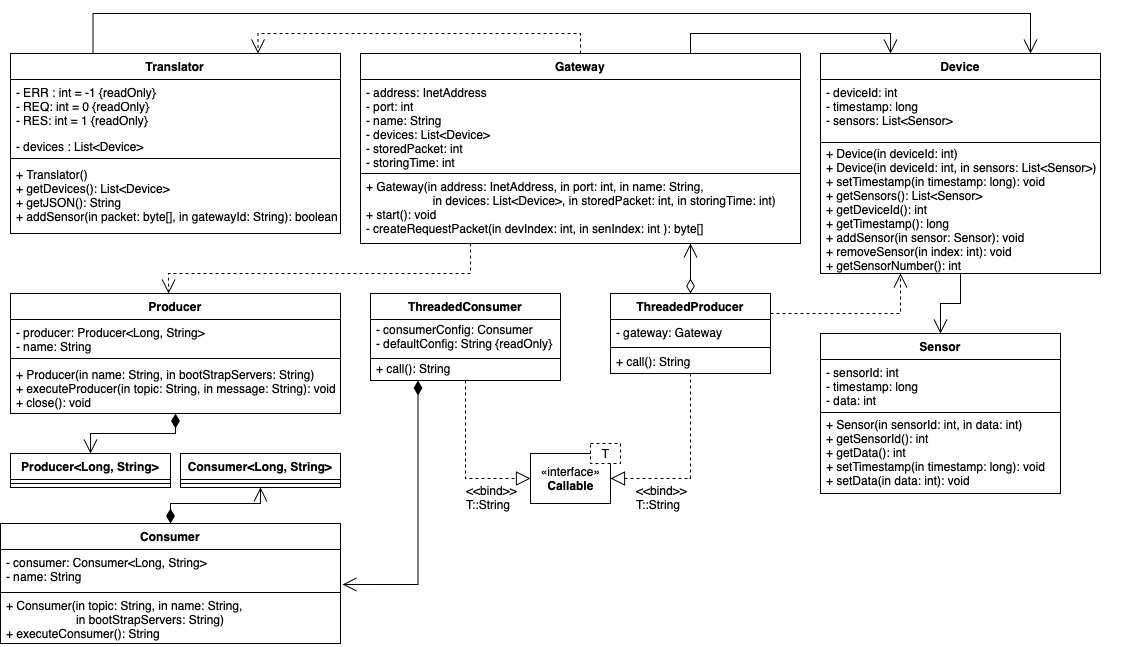
\includegraphics[scale=0.499]{res/images/GATEWAY/ClassiGateway.png}
				\caption{Diagramma delle classi per la componente gateway}
				\label{Diagramma 2}
			\end{figure}	
	\end{landscape}
		
	\begin{landscape}
		\subsubsection{Diagramma di sequenza}%%%%%%%%%%%%%%%%%%%%%%%OK
		  	\begin{figure}[H]
				\centering
				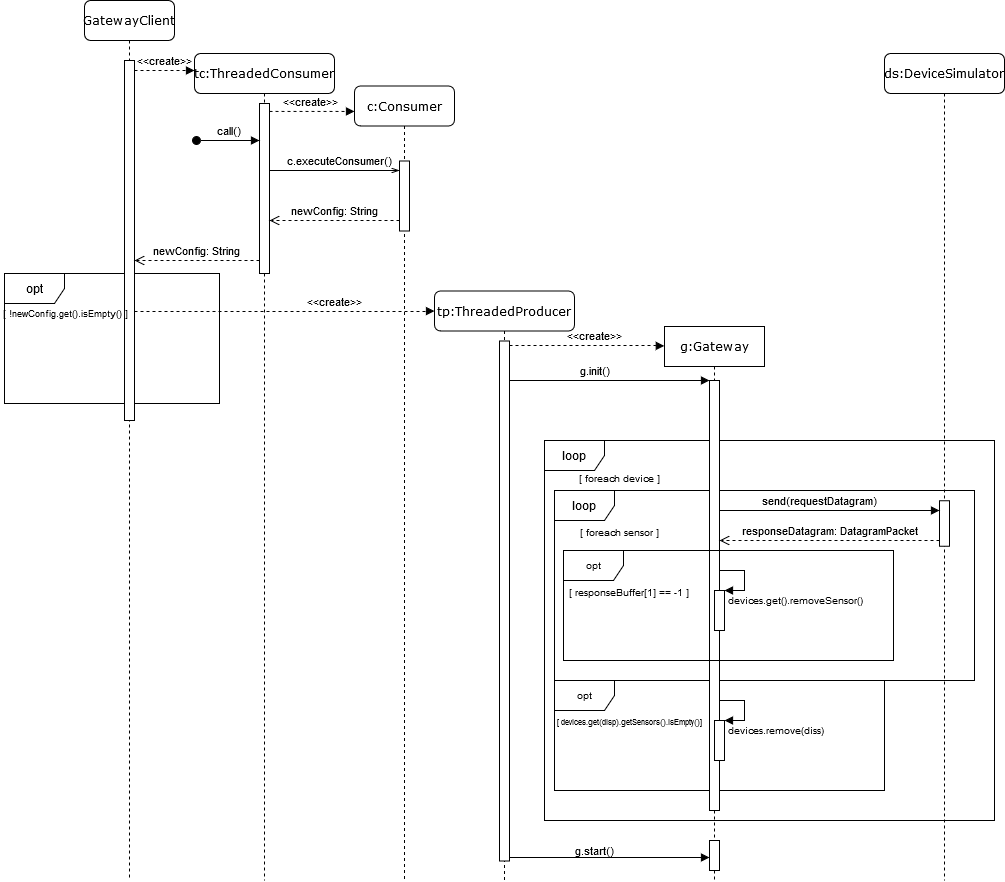
\includegraphics[scale=0.450]{res/images/GATEWAY/RichiestaInvioGateway.png}
				\caption{Diagramma di sequenza che rappresenta la richiesta di una prima configurazione ed un primo settaggio del gateway}
				\label{Diagramma 3}
			\end{figure}
	\end{landscape}
	
	\subsubsection{Diagramma di attività}%%%%%%%%%%%%%%OK
		\begin{figure}[H]
			\centering
			\includegraphics[scale=0.500]{res/images/GATEWAY/gateway.start().png}
			\caption{Diagramma di attività che rappresenta un'iterazione all'interno del metodo start() della classe gateway}
			\label{Diagramma 4}
		\end{figure}








